\section{Linear and Higher Order Approximations}\label{sec:Approx}
When we define the derivative $f^{\prime
}\left( x\right) $ as the rate of change of $f\left( x\right) $ with respect
to $x,$ we notice that in relation to the graph of $f,$ the derivative is
the slope of the tangent line, which (loosely speaking) is the line that just
grazes the graph. But what precisely do we mean by this? In short,
\textbf{the tangent line approximates the graph near the point of contact}. The
definition of the derivative $f^{\prime }\left( a\right) $ guarantees this
when it exists: By taking $x$ sufficiently close to $a$ but not equal to $a,$%
\begin{equation*}
\frac{f\left( x\right) -f\left( a\right) }{x-a}\approx f^{\prime }\left(
a\right) ,
\end{equation*}%
and consequently,%
\begin{equation*}
f\left( x\right) \approx f^{\prime }\left( a\right) \left( x-a\right)
+f\left( a\right) .
\end{equation*}%
The left hand side gives us the $y$-value of the function $y=f\left(
x\right) $ and the right hand side gives us the $y$-value $y=f^{\prime
}\left( a\right) \left( x-a\right) +f\left( a\right) $ for the tangent line
to the graph of $f$ at the point $\left( a,f\left( a\right) \right) .$

In this section we will explore how to apply this idea to approximate some
values of $f$, some changes in the values of $f$, and also the roots of $f.$

%%%%%%%%%%%%%%%%%%%%%%%%%%%%%%%%%%%%%%%%%%%%
% Subsections to include
%%%%%%%%%%%%%%%%%%%%%%%%%%%%%%%%%%%%%%%%%%%%
\subsection{Linear Approximations}\label{sec:LinApprox}
We begin by the first derivative as an application of the tangent line to approximate $f$.

Recall that the tangent line to $f(x)$ at a point $x=a$ is given by
\[ L(x) = f'(a) (x-a) + f(a).\]
The tangent line in this context is also called the \dfont{linear approximation} to $f$ at $a$.

If $f$ is differentiable at $a$ then $L$ is a good approximation of
$f$ so long as $x$ is ``not too far'' from $a$.  Put another way, if
$f$ is differentiable at $a$ then under a microscope $f$ will look
very much like a straight line, and thus will look very much like $L$;
since $L(x)$ is often much easier to compute than $f(x)$, then it makes sense to use $L$ as an approximation. Figure~\ref{fig:linear_approximation} 
shows a tangent line to $\ds y=x^2$ at three different magnifications. 

\figure[!ht]
\centerline{\includegraphics[width=2in]{images/linear_approx_1}\hfill
\includegraphics[width=2in]{images/linear_approx_2}\hfill
\includegraphics[width=2in]{images/linear_approx_3}\hfill}
\caption{The linear approximation to $\ds y=x^2$. \label{fig:linear_approximation}}
\endfigure

Thus in practice if we want to approximate a difficult value of $f(b)$,
then we may be able to approximate this value using a linear approximation,
provided that we can compute the tangent line at some point $a$ close to $b$.
Here is an example.

\begin{example}{Linear Approximation}{linear approximation}
Let $f(x)=\sqrt{x+4}$, what is $f(6)$?
\end{example}

\begin{solution}
We are asked to calculate $f(6)=\sqrt{6+4}=\sqrt{10}$ which is not easy
to do without a calculator. However 9 is (relatively) close to 10 and
of course $f(5)=\sqrt{9}$ is easy to compute, and we use this to approximate $\sqrt{10}$.

To do so we have $f'(x)=1/(2\sqrt{x+4})$, and thus the linear approximation to $f$ at $x=5$ is
\[L(x)=\bigg(\frac{1}{2\sqrt{5+4}}\bigg)(x-5)+\sqrt{5+4}=\frac{x-5}{6}+3.\]

Now to estimate $\sqrt{10}$, we substitute 6 into the linear approximation $L(x)$ instead of $f(x)$, to obtain
\[ \sqrt{6+4}\approx \frac{6-5}{6}+3=\frac{19}{6}=3\sfrac{1}{6}=3.1\bar{6}\approx 3.17 \]

It turns out the exact value of $\sqrt{10}$ is actually 3.16227766\ldots
but our estimate of 3.17 was very easy to obtain and is relatively accurate.
This estimate is only accurate to one decimal place.
\end{solution}
 
With modern calculators and computing software it may not appear
necessary to use linear approximations, but in fact they are quite
useful. For example in cases requiring an explicit numerical approximation, they
allow us to get a quick estimate which can be used as a
``reality check'' on a more complex calculation. Further in some complex
calculations involving functions, the linear approximation makes an
otherwise intractable calculation possible without serious loss of
accuracy.

\begin{example}{Linear Approximation of Sine}{linear approximation of sine}
Find the linear approximation of $\sin x$ at $x=0$, and use it to compute small values of $\sin x$.
\end{example}

\begin{solution}
If $f(x)=\sin x$, then $f'(x)=\cos x$, and thus the linear approximation of $\sin x$ at $x=0$ is:
\[ L(x)=\cos (0)(x-0)+\sin (0)=x. \]
Thus when $x$ is small this is quite a good approximation and is used
frequently by engineers and scientists to simplify some calculations.

For example you can use your calculator (in radian mode since the
derivative of $\sin x$ is $\cos x$ only in radian) to see that
\[ \sin (0.1)=0.099833416\ldots \]
and thus $L(0.1)=0.1$ is a very good and quick approximation without any calculator!
\end{solution}


%%%%%%%%%%%%%%%%%%%%%%%%%%%%%%%%%%%%%%%%%%%%%%%
\Opensolutionfile{solutions}[ex]
\section*{Exercises for \ref{sec:LinApprox}}

\begin{enumialphparenastyle}

%%%%%%%%%%
\begin{ex} 
Find the linearization $L(x)$ of $f(x)=\ln (1+x)$ at $a=0$. Use
this linearization to approximate $f(0.1)$.
\begin{sol}
$L(x)=x$, $f(0.1)\approx L(0.1)=0.1$
\end{sol}
\end{ex}

%%%%%%%%%%
\begin{ex} 
Use linear approximation to estimate $(1.9)^3$.
\begin{sol}
Choose $f(x)=x^3$ and $a=2$, the closest integer to 1.9. The
linearization of $f$ at $a$ is $L(x)=12(x-2)+8$, and $(1.9)^3=f(1.9)\approx L(1.9)=12(1.9-2)+8=6.8$.
\end{sol}
\end{ex}

%%%%%%%%%%
\begin{ex} 
Show in detail that the linear approximation of
$\sin x$ at $x=0$ is $L(x)=x$ and the linear approximation of $\cos x$
at $x=0$ is $L(x)=1$.
\end{ex}

%%%%%%%%%%
\begin{ex} 
Use $f(x)=\sqrt[3]{x+1}$ to approximate $\sqrt[3]{9}$ by choosing an
appropriate point $x=a$. Are we over- or under-estimating the value of $\sqrt[3]{9}$? Explain.
\begin{sol}
Choose $a=7$ since $f(7)=\sqrt[3]{7+1}=\sqrt[3]{8}=2$ is an integer
close to $\sqrt[3]{9}$. The linearization of $f$ at $a=7$ is
$L(x)=\sfrac{1}{12}(x-7)+2$. Then $f(8)=\sqrt[3]{8+1}=\sqrt[3]{9}\approx L(8)=\sfrac{1}{12}(8-7)+2=2.08\bar{3}$. We are over-estimating $\sqrt[3]{9}$ since $L(x)>f(x)$ for all $x$ around $a=7$.
\end{sol}
\end{ex}

\end{enumialphparenastyle}
\subsection{Differentials}\label{sec:differentials}
Very much related to linear approximations are the {\em differentials} $dx$ and $dy$, used not to approximate values of $f$, but instead the change (or rise) in the values of $f$.

\begin{definition}{Differentials dx and dy}{dx}
Let $y=f(x)$ be a differentiable function. We define a new
  independent variable $dx$, and a new dependent variable
  $dy=f'(x)\,dx$. Notice that $dy$ is a function both of $x$ (since
  $f'(x)$ is a function of $x$) and of $dx$.  We call both $dx$ and
  $dy$ \deffont{differentials}.  
\end{definition}

Now fix a point $a$ and let $\Delta x =x-a$ and $\Delta y= f(x)-f(a)$.
If $x$ is near $a$ then $\Delta x$ is clearly small. If we set $dx=\Delta x$ then we obtain
\[ dy = f'(a)\,dx \approx \frac{\Delta y}{\Delta x}\Delta x = \Delta y.\]
Thus, $dy$ can be used to approximate $\Delta y$, the actual change in
the function $f$ between $a$ and $x$. This is exactly the
approximation given by the tangent line:
\[ dy = f'(a)(x-a) = f'(a)(x-a)+f(a)-f(a)=L(x)-f(a).\]
While $L(x)$ approximates $f(x)$, $dy$ approximates how $f(x)$ has
changed from $f(a)$.
Figure~\ref{fig:differentials} illustrates the relationships.

\figure[!ht]
\centerline{\vbox{\beginpicture
\normalgraphs
%\sevenpoint
\setcoordinatesystem units <2truecm,2truecm>
\setplotarea x from 0 to 4.5, y from 0 to 2.5
\axis left /
\axis bottom ticks withvalues {$a$} {$x$} / at 1 3 / /
\plot 0.500 0.707 0.588 0.766 0.675 0.822 0.762 0.873 0.850 0.922 
0.938 0.968 1.025 1.012 1.112 1.055 1.200 1.095 1.288 1.135 
1.375 1.173 1.462 1.209 1.550 1.245 1.638 1.280 1.725 1.313 
1.812 1.346 1.900 1.378 1.988 1.410 2.075 1.440 2.162 1.471 
2.250 1.500 2.338 1.529 2.425 1.557 2.512 1.585 2.600 1.612 
2.688 1.639 2.775 1.666 2.862 1.692 2.950 1.718 3.038 1.743 
3.125 1.768 3.212 1.792 3.300 1.817 3.388 1.841 3.475 1.864 
3.562 1.887 3.650 1.910 3.738 1.933 3.825 1.956 3.912 1.978 
4.000 2.000 /
\setlinear
\plot 1 1 3 2 3 1 1 1 /
\betweenarrows {$dx=\Delta x$} from 1 0.8 to 3 0.8
\betweenarrows {$\Delta y$} from 3.2 1 to 3.2 1.73
\betweenarrows {$dy$} from 3.6 1 to 3.6 2
\setdashes <2pt>
\putrule from 3 2 to 3.6 2
\putrule from 3 1 to 3.6 1
\putrule from 3 1.73 to 3.2 1.73
\endpicture}}
\caption{Differentials.\label{fig:differentials}}
\endfigure

Here is a concrete example.

\begin{example}{Rise of Natural Logarithm}{rise of natural logarithm}
Approximate the rise of $f(x)=\ln x$ from $x=1$ to $x=1.1$, using linear approximation.
\end{example}

\begin{solution}
Note that $\ln (1.1)$ is not readily calculated (without a calculator) hence why we wish to use linear approximation to approximate $f(1.1)-f(1)$.

We fix $a=1$ and as above we have $\Delta x=x-1$ and $\Delta y=f(x)-f(1)=\ln x$, and obtain
\[ dy=f'(1)dx\approx \frac{\Delta y}{\Delta x}\Delta x=\Delta y. \]
But $f'(x)=1/x$ and thus $f'(1)=1/1=1$, we obtain in this case
\[ dy=dx\approx\Delta y. \]
Finally for $x=1.1$, we can easily approximate the rise of $f$ as
\[ f(1.1)-f(1)=\Delta y\approx dy=1.1-1=0.1. \]
The correct value of $\ln (1.1)=\ln 1$ is 0.0953\ldots and thus we were relatively close.
\end{solution}


%%%%%%%%%%%%%%%%%%%%%%%%%%%%%%%%%%%%%%%%%%%%%%%
\Opensolutionfile{solutions}[ex]
\section*{Exercises for \ref{sec:differentials}}

\begin{enumialphparenastyle}
	
%%%%%%%%%%
\begin{ex} 
Let $\ds f(x) = x^4$. If $a=1$ and $dx= \Delta x =1/2$, 
what are $\Delta y$ and $dy$?
\begin{sol}
	$\Delta y=65/16$, $dy=2$
\end{sol}
\end{ex}

%%%%%%%%%%
\begin{ex} 
Let $\ds f(x) = \sqrt{x}$. If $a=1$ and $dx= \Delta x
=1/10$, what are $\Delta y$ and $dy$?
\begin{sol}
	$\ds \Delta y=\sqrt{11/10}-1$, $dy=0.05$
\end{sol}
\end{ex}

%%%%%%%%%%
\begin{ex} 
Let $f(x) = \sin (2x)$. If $a=\pi$ and $dx= \Delta x
=\pi/100$, what are $\Delta y$ and $dy$?
\begin{sol}
	$\ds \Delta y=\sin(\pi/50)$, $dy=\pi/50$
\end{sol}
\end{ex}

%%%%%%%%%%
\begin{ex} 
Use differentials to estimate the amount of paint needed to
 apply a coat of paint 0.02 cm thick to a sphere with diameter $40$
 meters. (Recall that the volume of a sphere of radius $r$ is $V
 =(4/3)\pi r^3$. Notice that you are given that $dr=0.02$.)
\begin{sol}
	$dV=8\pi/25$
\end{sol}
\end{ex}

\end{enumialphparenastyle}
\subsection{Taylor Polynomials}\label{sec:Taylor}
We can go beyond first order derivatives to create polynomials approximating a function as closely as we wish, these are called $Taylor$ $Polynomials$.

While our linear approximation $L(x)=f'(a)(x-a)+f(a)$ at a point $a$ was a polynomial of degree 1 such that both $L(a)=f(a)$ and $L'(a)=f'(a)$, we can now form a polynomial
\[ T_n(x)=a_0+a_1(x-a)+a_2(x-a)^2+a_3(x-a)^3+\dots +a_n(x-a)^n \]
which has the same first $n$ derivatives at $x=a$ as the function $f$.

By successively computing the derivatives of $T_n$, we obtain:
\[ \begin{array}{l}
a_0 = f(a)=\frac{f(a)}{0!}\\
a_1 = \frac{f'(a)}{1!}\\
a_2 = \frac{f''(a)}{2!}\\
\cdots \\
a_k = \frac{f^{(k)}(a)}{k!}\\
\cdots a_n =\frac{f^{(n)}(a)}{n!}
\end{array} \]
where $f^{(k)}(x)$ is the $k^{th}$ derivative of $f(x)$, and
$n!=n(n-1)(n-2)\ldots (2)(1) $, referred to as \ifont{factorial} notation.

Here is an example.

\begin{example}{Approximate e using Taylor Polynomials}{approximate e using taylor polynomials}
Approximate $e^x$ using Taylor polynomials at $a=0$, and use this to approximate $e$.
\end{example}

\begin{solution}
In this case we use the function $f(x)=e^x$ at $a=0$, and therefore
\[ T_n(x)=a_0+a_1x+a_xx^2+a_3x^3+\ldots +a_nx^n \]

Since all derivatives $f^{(k)}(x)=e^x$, we get:
\[ \begin{array}{l}
a_0=f(0)=1 \\
a_1=\frac{f'(0)}{1!}=1 \\
a_2=\frac{f''(0)}{2!}=\frac{1}{2!} \\
a_3=\frac{f'''(0)}{3!}=\frac{1}{3!} \\
\cdots \\
a_k=\frac{f^{(k)}(0)}{k!}=\frac{1}{k!} \\
\cdots \\
a_n=\frac{f^{(n)}(0)}{n!}=\frac{1}{n!} 
\end{array} \]
Thus
\[ \begin{array}{l}
T_1(x)=1+x=L(x) \\
T_2(x)=1+x+\frac{x^2}{2!} \\
T_3(x)=1+x+\frac{x^2}{2!}+\frac{x^3}{3!}
\end{array} \]
and in general
\[ T_n(x)=1+x+\frac{x^2}{2!}+\frac{x^3}{3!}+\cdots +\frac{x^n}{n!}. \]

Finally we can approximate $e=f(1)$ by simply calculating $T_n(1)$. A few values are:
\[ \begin{array}{l}
T_1(1)=1+1=2 \\
T_2(1)=1+1+\frac{1^2}{2!}=2.5 \\
T_4(1)=1+1+\frac{1^2}{2!}+\frac{1^3}{3!}=2.\overline{6} \\
T_8(1)=2.71825396825 \\
T_{20}(1)=2.71828182845
\end{array} \]

We can continue this way for larger values of $n$, but $T_{20}(1)$ is already a pretty good approximation of $e$, and we took only 20 terms!
\end{solution}
%
%\subsubsection{Taylor's Theorem}\label{subsubsec:TaylorsTheoremsubsubsec}
%We have now seen how a polynomial is used to approximate a function $f$ near $a$. But how close is our approximation to the actual function? That is to say, can we measure the error in our approximation?
%
%\begin{theorem}{Taylor's Theorem}{TaylorTheorem}
%Suppose $f$ is defined and has $n+1$ continuous derivatives on an open interval $I$ containing $a$. Then for each $x$ in the interval,
%\[\ds f(x)=\left[\sum_{k=0}^n\frac{f^{(k)}(a)}{k!}(x-a)^k\right]+R_{n+1}(x)\]
%where the error term is 
%\[R_{n+1}(x)=\frac{f^{(n+1)}(z)}{(n+1)!}(x-a)^{n+1}\]
%for some $z$ between $a$ and $x$.
%\end{theorem}
%
%The form for the error $R_{n+1}(x)$ is called the \dfont{Lagrange Formula} for the remainder. Notice that this error term looks quite similar to how we would expect the next term in the Taylor Polynomial of $f(x)$ to look. The main difference is that $f^{(n+1)}$ is evaluated at a point $z$ and not necessarily at the center $a$, and we do not know what $z$ might be.
%
%Notice as well that when $n=0$, Taylor's Theorem is precisely the Mean Value Theorem, which is mainly how we would prove Taylor's Theorem (but will not prove here). The following corollary is useful when applying the theorem.
%
%\begin{corollary}{Corollary to Taylor's Theorem}{TaylorTheoremCorollary}
%Let $\mu_{n+1}$ be the maximum of $|f^{(n+1)}(x)|$ on some interval containing the center $a$. Then for any $x$ in this interval, the error of the Taylor Polynomial is bounded as follows.
%\[\ds |f(x)-T_n(x)|\leq \frac{\mu_{n+1}}{(n+1)!}|x-a|^{n+1}.\]
%\end{corollary}
%
%Observe that if $f^{(n+1)}(x)=0$, then the Taylor Polynomial of degree $n$ is an exact approximation of the function $f$. Why? If the $(n+1)$\textsuperscript{th} derivative of a function is 0, then $f$ is simply a polynomial of degree at most $n$.
%
%Let's look at an example:
%
%\begin{example}{Approximate Square Root}{ApproxSquareRootTaylorTheorem}
%Approximate $\sqrt{11}$ to accuracy of at least 0.01.
%\end{example}
%\begin{solution}
%The 2nd degree Taylor Polynomial of $f(x)=\sqrt{x}$ centered at $x=9$ is given by:
%\[\ds T_2(x)=3+\frac{1}{6}(x-9)-\frac{1}{216}(x-9)^2.\]
%For our purposes a 2nd degree polynomial should be sufficient to produce our desired level of accuracy, which we will see shortly. If we require greater accuracy, we can simply increase the degree of the Taylor Polynomial. At $x=11$ this polynomial approximation gives $T_2(10)=3.3\overline{148}$.
%
%Now we must determine the accuracy of our approximation. We first find that the third derivative of $\sqrt{x}$ if $f'''(x)=\frac{3}{8}x^{-5/2}$, and that this function's maximum in the interval $[9,11]$ occurs at $x=9$ (since it is a positive decreasing function). Thus, the maximum value is $\mu_3=f'''(9)=\frac{3}{8}\cdot\frac{1}{243}=\frac{3}{1944}=\frac{1}{648}$. Applying the corollary we get
%\begin{align*}
%\left|\sqrt{11}-3.3\overline{148}\right|&\leq\frac{1}{648}\frac{1}{3!}(11-9)^3	\\
%&\leq\frac{1}{486}\approx 0.0020576
%\end{align*}
%Therefore, the approximation $3.3\overline{148}$ is guaranteed to be accurate to at least $\frac{1}{486}$, which is less than 0.01.
%\end{solution}


%%%%%%%%%%%%%%%%%%%%%%%%%%%%%%%%%%%%%%%%%%%%%%%
\Opensolutionfile{solutions}[ex]
\section*{Exercises for \ref{sec:Taylor}}

\begin{enumialphparenastyle}

%%%%%%%%%%
\begin{ex} 
Find the 5\textsuperscript{th} degree Taylor polynomial for $f(x)=\sin x$ around $a=0$.
\begin{enumerate}
	\item	Use this Taylor polynomial to approximate $\sin (0.1)$.
	\item	Use a calculator to find $\sin (0.1)$. How does this compare to our approximation in part (a)?
\end{enumerate}
\begin{sol}
$T_5(x)=x-\frac{x^3}{3!}+\frac{x^5}{5!}$
\begin{enumerate}
	\item	$\sin (0.1)\approx T_5(0.1)\approx 0.10016675$
	\item	$\sin (0.1)=0.0998334\ldots$ using a calculator. Our approximation is accurate to $0.10016675-0.0998334\ldots =0.000\bar{3}$.
\end{enumerate}
\end{sol}
\end{ex}


%%%%%%%%%%
\begin{ex}
Suppose that $f^{\prime\prime}$ exists and is continuous on $[1,2]$.
Suppose also that $\left\vert f^{\prime\prime}(x)\right\vert \leq \frac{1}{4}$
for all $x$ in $(1,2)$. Prove that if we use the linearization $y=L(x)$
of $y=f(x)$ at $x=1$ as an approximation of $y=f(x)$ near $x=1$,
then our estimated value of $f(1.2)$ is
guaranteed to have an accuracy of at least 0.01, i.e., our estimate will lie
within 0.01 units of the true value.
\end{ex}


%%%%%%%%%%
\begin{ex} 
Find the 3\textsuperscript{rd} degree Taylor polynomial for $f(x)=\frac{1}{1-x}-1$ around $a=0$. Explain why this approximation would not be useful for calculating $f(5)$.
\begin{sol}
	$T_3(x)=x+x^2+x^3$. The point $x=5$ is not close to $x=0$, and $f$ is not continuous at $x=1$.
\end{sol}
\end{ex}

%%%%%%%%%%
\begin{ex} 
Consider $f(x)=\ln x$ around $a=1$.
\begin{enumerate}
	\item	Find a general formula for $f^{(n)}(x)$ for $n\geq 1$.
	\item	Find a general formula for the Taylor Polynomial, $T_n(x)$.
\end{enumerate}
\begin{sol}
\begin{enumerate}
	\item	$f^{(n)}(x)=\frac{(-1)^{(n-1)}(n-1)!}{x^n}$
	\item	$T_n(x)=\ln (1)+\displaystyle\sum_{i=1}^{n} \frac{\big(\frac{(-1)^{(i-1)}(i-1)!}{1^n}\big)}{i!}(x-1)^i=\displaystyle\sum_{i=1}^{n} \bigg(\frac{(-1)^{(i-1)}(i-1)!}{i!}\bigg)(x-1)^i$ since $\ln (1)=0$ and $1^n=1$.
\end{enumerate}
\end{sol}
\end{ex}

%% % % % % % % % % %
%% Exercises for Taylor's Theorem
%% % % % % % % % % %
%\begin{ex}
%Approximate $\ln(1.3)$ to accuracy of at least 0.0001.
%\end{ex}
%
%\begin{ex}
%Determine a general inequality describing the error of Taylor Polynomial approximations of $f(x)=\sin(x)$ and $g(x)=\cos(x)$. \ifont{(Hint: Build the inequality in Corollary~\ref{cor:TaylorTheoremCorollary})}
%\begin{sol}
%	\begin{align*}
%	|\sin(x)-T_n(x)|&\leq\frac{1}{(n+1)!}x^{n+1}	\\
%	|\cos(x)-T_n(x)|&\leq\frac{1}{(n+1)!}x^{n+1}
%	\end{align*}
%\end{sol}
%\end{ex}
%
%% % % % % % % % % %

\end{enumialphparenastyle}
\subsection{Newton's Method}\label{sec:Newton}
A well known numeric method is \ifont{Newton's Method} (also sometimes
referred to as \ifont{Newton-Raphson's Method}), named after Isaac Newton
and Joseph Raphson.  This method is used to find roots, or
$x$-intercepts, of a function.  While we may be able to find the roots
of a polynomial which we can easily factor, we saw in the previous
chapter on {\bf Limits}, that for example the function $e^x + x = 0$
has a solution ($i.e.$ root, or $x$-intercept) at $x \approx
-0.56714$.  By the \ifont{Intermediate Value Theorem} we know that the
function $e^x + x = 0$ does have a solution. We cannot here simply
solve for such a root algebraically, but we can use a numerical method
such as $Newton's$.  Such a process is typically classified as an
$iterative$ method, a name given to a technique which involves
repeating similar steps until the desired accuracy is obtained.   Many
computer $algorithms$ are coded with a for-loop, repeating an
iterative step to converge to a solution.

The idea is to start with an initial value $x_0$ (approximating the
root), and use linear approximation to create values $x_1$, $x_2$, $\cdots$ getting closer and closer to a root. 

The first value $x_1$ corresponds to the intercept of the tangent line
of $f(x_0)$ with the $x$-axis, which is:
\[ x_1 = x_0 -\frac{f(x_0)}{f'(x_0)} \]

\figure[!ht]
$$\includegraphics[width=1.75in]{images/newton_figure_1}$$
\caption{First iteration of Newton's Method. \label{fig:Newton1}} 
\endfigure

We can see in Figure~\ref{fig:Newton1}, that if we compare the point $(x_0,0)$ to
$(x_1,0)$, we would likely come to the conclusion that $(x_1,0)$ is
closer to the actual root of $f(x)$ than our original guess,
$(x_0,0)$.  As will be discussed, the choice of $x_0$ must be done
correctly, and it may occur that $x_1$ does not yield a better
estimate of the root.

Newton's method is simply to repeat this process again and again 
in an effort to obtain a more accurate solution.  Thus at the next step we obtain:

\[ x_2 = x_1 -\frac{f(x_1)}{f'(x_1)} \]

\figure[!ht]
$$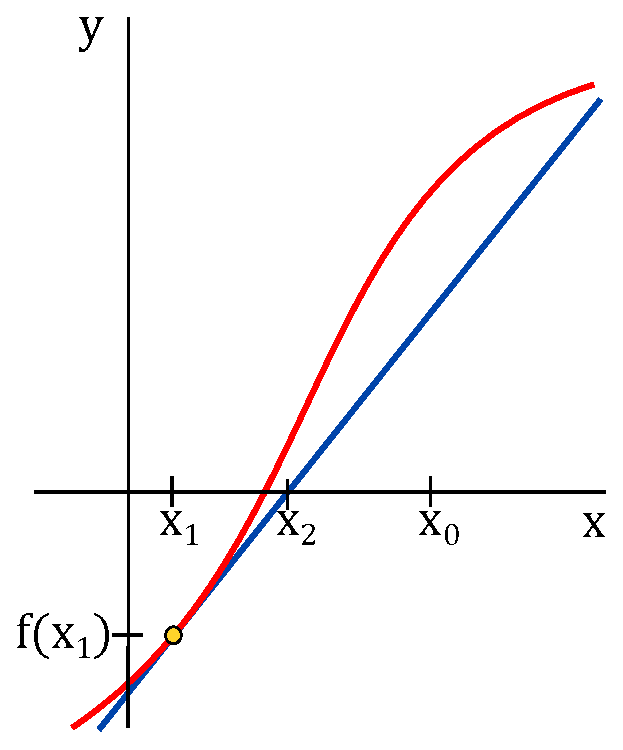
\includegraphics[width=1.75in]{images/newton_figure_2}$$
\caption{Second iteration of Newton's Method. \label{fig:Newton2}}
\endfigure

We can now clearly see how $(x_2,0)$ is a better estimate of the root
of $f(x)$, rather than any of the previous points.  Moving forward, we
will get:
\[ x_3 = x_2 -\frac{f(x_2)}{f'(x_2)} \]
Rest assured, $(x_3,0)$ will be an even better estimate of the root!  We express the general iterative step as:
\[ x_{n+1} = x_n -\frac{f(x_n)}{f'(x_n)} \]

The idea is to iterate these steps to obtain the desired accuracy. Here is an example. 

\begin{example}{Newton method to approximate roots}{newtonroot}
Use Newton's method to approximate the roots of $f(x)=x^3-x+1$.
\end{example}

\begin{solution}
You can try to find solve the equation algebraically to see that this
is a difficult task, and thus it make sense to try a numerical method
such as Newton's.

To find an initial value $x_0$, note that $f(-1)=-5$ and $f(0)=1$,
and by the Intermediate Value Theorem this $f$ has a root between these two values, and we decide to start with $x_0=-1$ (you can try other values to see what happens).

Note that $f'(x)=3x^2-1$, and thus we get
\[ x_{n+1} = x_n -\frac{f(x_n)}{f'(x_n)} = x+n - \frac{x^3_n-x_n+1}{3x^2_n-1} \]
Thus we can produce the following values (try it):
\[ \begin{array}{l}
x_0 = -1 \\
x_1= -1.5000\\
x_2 = -1.347826.. \\
x_3= -1.325200.. \\
x_4 = -1.324718.. \\
x_5 = -1.324717..  \\
x_6 = -1.324717..  \\
\cdots
\end{array} \]
and we can now approximate the root as $-1.324717$.
\end{solution}

As with any numerical method, we need to be aware of the weaknesses of
any technique we are using.

\figure[!ht]
$$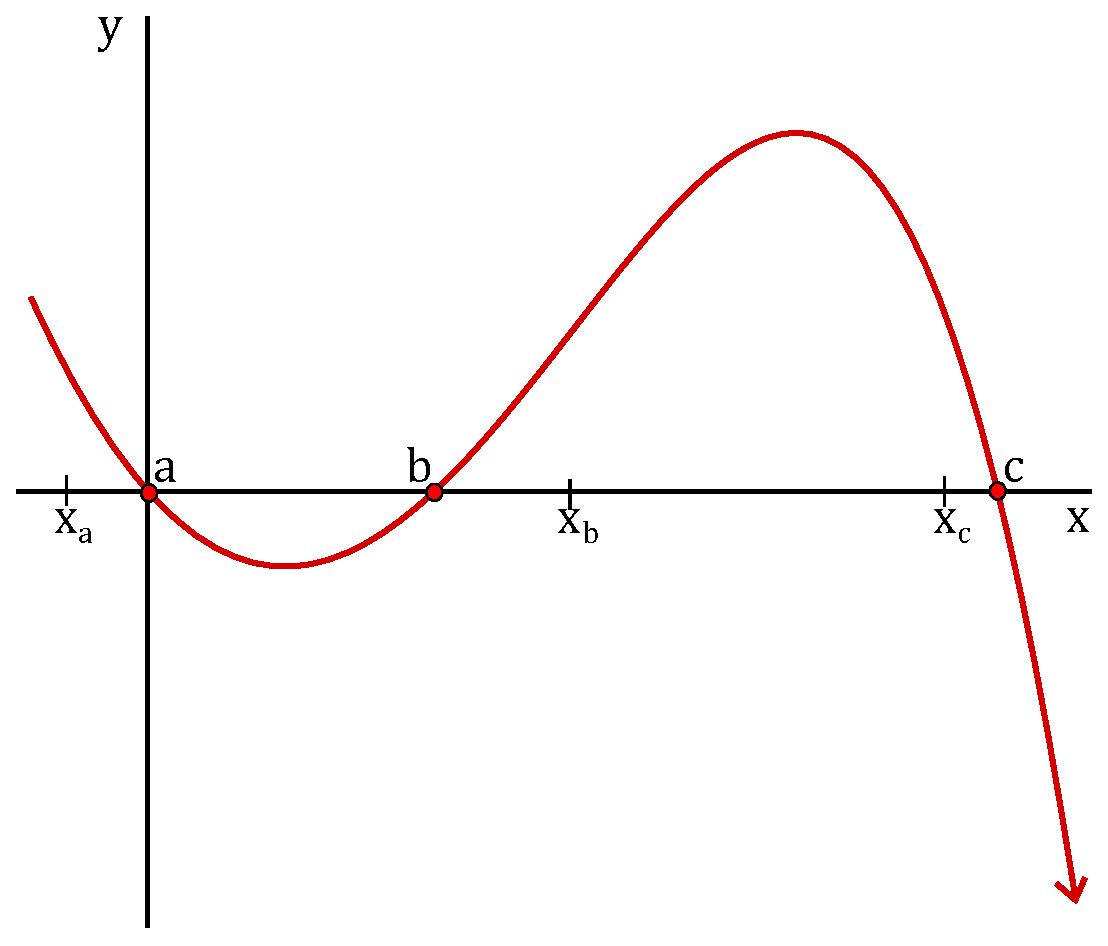
\includegraphics[width=2.5in]{images/newton_figure_4}$$
\caption{Function with three distinct solutions. \label{fig:Newton4}}
\endfigure

%% need an easy example here

If we know our root is somewhere near $a$, we would make our guess
$x_0=a$.  Generally speaking, a good practice is to make our guess as
close to the actual root as possible. In some cases we may have no idea where the root is, so it would be prudent to
perform the algorithm several times on several different initial
guesses and analyze the results. 

For example we can see in Figure~\ref{fig:Newton4} that $f(x)$ in fact has three roots, and depending on our initial
guess, we may get the algorithm to converge to different roots.  If we
did not know where the roots were, we would try the technique several
times.  In one instance, if our initial guess was $x_a$, we'd
likely converge to $(a, 0)$.  Then if we were to choose another
guess, $x_b$, then we'd likely converge to $(b, 0)$.
Eventually, using various initial guesses we'd get one of three roots:
$a$, $b$, or $c$.  Under these circumstances we can
clearly see the effectiveness of this numeric method.

\figure[!ht]
$$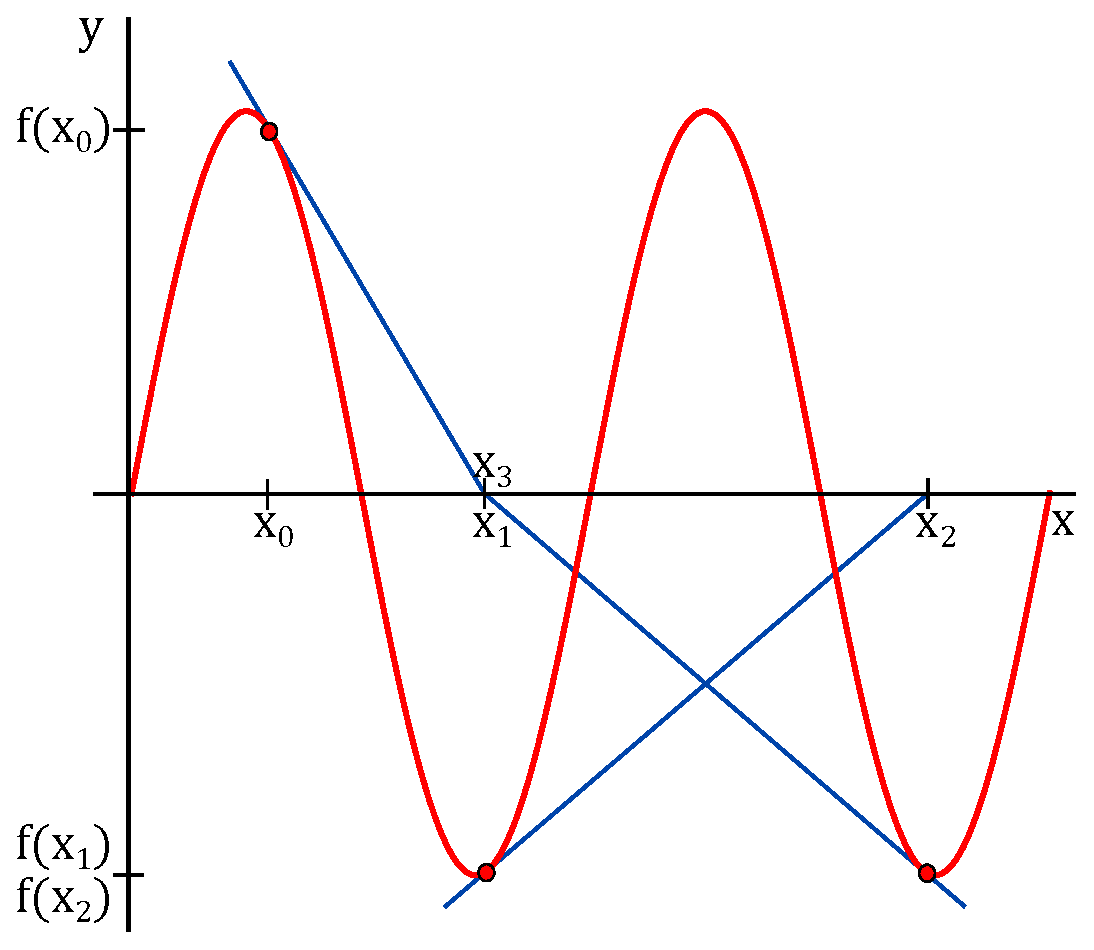
\includegraphics[width=3.5in]{images/newton_figure_3}$$
\caption{Newton's Method applied to $\sin x$. \label{fig:Newton3}}
\endfigure

As another example if we attempt to use $Newton's$ $Method$ on $f(x) =
\sin x$ using $x_0=\pi/2$, then $f'(x_0)=0$ so $x_1$ is undefined and we cannot proceed. 
Even in general $x_{n+1}$ is typically nowhere near $x_n$,
and in general not converging to the root nearest to our initial guess
of $x_0$.  In effect, the algorithm keeps "bouncing around". An example of which is depicted in Figure~\ref{fig:Newton3}. Based on
our initial guess for such a function, the algorithm may or may not
converge to a root, or it may or may not converge to the root {\bf
closest} to the initial guess.  This gives rise to the more common
issue: Selection of the initial guess, $x_0$.

Here is a summary.

{\bf Key Points in using Newton's method to approximate a root of $f(x)$}

\begin{enumerate}
\item Choosing $x_0$ as close as possible to the root we wish to find.
\item A guess for $x_0$ which makes the algorithm ``bounce around'' is considered $unstable$.
\item Even the smallest changes to $x_0$ can have drastic effects: We may converge to another root, 
we may converge very slowly (requiring many more iterations), or we may encounter an unstable point.
\item We may encounter a $stationary$ $point$ if we choose $x_0$ such that $f'(x)=0$ ($i.e.$ at a critical point!) in which case the algorithm fails.
\end{enumerate}

This is all to say that your initial guess for $x_0$ can be extremely
important.


%%%%%%%%%%%%%%%%%%%%%%%%%%%%%%%%%%%%%%%%%%%%%%%
\Opensolutionfile{solutions}[ex]
\section*{Exercises for \ref{sec:Newton}}

\begin{enumialphparenastyle}

%%%%%%%%%%
\begin{ex} 
Use Newton's Method to find all roots of $f(x)=3x^2-9x-11$. (Hint: use Intermediate Value Theorem to choose an appropriate $x_0$)
\begin{sol}
	Notice that $f(-2)=19$, $f(0)=-11$, and $f(5)=19$ and $f$ is a continuous function. By the
	Intermediate Value Theorem there exists a root in $[-2,0]$ and $[0,5]$. Choose $x_0=0$, then $x_4\approx -0.93242$.
	Choose $x_0=5$, then $x_4\approx 3.93242$.
\end{sol}
\end{ex}

%%%%%%%%%%
\begin{ex} 
Consider $f(x)=x^3-x^2+x-1$.
\begin{enumerate}
	\item	Using initial approximation $x_0=2$, find $x_4$.
	\item	What is the exact value of the root of $f$? How does this compare to our approximation $x_4$ in part (a)?
	\item	What would happen if we chose $x_0=0$ as our initial approximation?
\end{enumerate}
\begin{sol}
\begin{enumerate}
	\item	$x_4\approx 1.00022\ldots$
	\item	$x=1$ is the root of $f$. Our approximation in part (a) was correct to 3 decimal places.
	\item	$x_1=1$. The root is found in one iteration of Newton's Method.
\end{enumerate}
\end{sol}
\end{ex}

%%%%%%%%%%
\begin{ex} 
Consider $f(x)=\sin x$. What happens when we choose $x_0=\pi/2$? Explain.
\begin{sol}
	$\cos (\pi/2)=0$, so $x_1$ is undefined.
\end{sol}
\end{ex}

\end{enumialphparenastyle}

% Exercises for each subsection are in the separate files